\section{Lógica matemática}


    Muchos algoritmos y demostraciones usan expresiones lógicas tales como
    \texttt{si p entonces q}. Por tanto, es necesario conocer los casos en los cuales esas expresiones son \texttt{ciertas} o \texttt{falsas}. Discutiremos esto en esta unidad. 

    También investigamos el valor de verdad de enunciados cuantificados, que son aquellos que usan los cuantificadores lógicos \texttt{para todo...} y \texttt{existe...}
    \marginnote{    	En este curso, usaremos el \emph{sistema algebraico de computo} \texttt{SageMath}, el cuál está escrito con base en el lenguaje de programación \texttt{Python} e incorpora diversos paquetes de \texttt{OpenSource}.  
    	Puede acceder a este sistema, a través de \href{https://cloud.sagemath.com/}{https://cloud.sagemath.com/} }


\subsection{Proposiciones y Declaraciones Compuestas}

    Una proposición es un enunciado declarativo que puede ser cierto o falso, pero no ambos. 

    \begin{resuelto}
        ?`Cuál de los siguientes enunciados es una proposición?
        \begin{multicols}{2}
            \begin{enumerate}
                \item El hielo flota en el agua.
                \item China está en Europa.
                \item $2+2=4$
                \item $2+2=5$
                \item ?`A donde vas?
                \item Haz tu tarea.
            \end{enumerate}
        \end{multicols}
    \end{resuelto}
    


\subsection{Proposiciones compuestas}


    Muchas proposiciones están \texttt{compuestas} de proposiciones más simples, llamadas \emph{subproposiciones}, por medio de \emph{conectores lógicos.}  Una proposición se dice que es \emph{primitiva} si no puede descomponerse en proposiciones más simples.



    Por ejemplo, las siguientes proposiciones son compuestas
    \begin{itemize}
        \item ``Hoy lloverá y hará mucho frío.''
        \item ``Ahorro para salir de viaje o compró un televisor nuevo.''
    \end{itemize}
    



    La propiedad fundamental de una proposición compuesta es que su valor de verdad está completamente determinado por los valores de verdad de sus subproposiciones y la manera en la cual están conectadas para formar la proposición compuesta. 


    En esta sección discutiremos las tres operaciones lógicas básicas: conjunción , disyunción  y la negación.


\subsection{Conjunción}


    Cualesquiera dos proposiciones $p,q$ pueden ser combinadas por la palabra ``y'' para formar una proposición compuesta llamada \emph{conjunción} que se escribe $p\wed q.$



    \begin{definicion}
        Si tanto $p$ como $q$ son ciertas, entonces $p \wed q$ es cierta; en otro caso $p\wed q$ es falsa.
        \sidenote{
        	\begin{tdv}[Conjunción]\hfill
        		\label{tdv:and}
        		\begin{center}
        			\begin{tabular}{|l|l|l|}\hline
        				$p$ & $q$ & $p \wed q$\\\hline
        				1 & 1 & 1\\\hline
        				1 & 0 & 0\\\hline
        				0 & 1 & 0\\\hline
        				0 & 0 & 0\\\hline
        			\end{tabular}
        		\end{center}        
        	\end{tdv}
        }  
    \end{definicion}	

    \begin{observacion}
        Para entender mejor como se conectan los valores de verdad, generalmente se utilizan \emph{tablas de verdad.}  
        
        Por brevedad $1$ representará el valor \texttt{cierto}, mientras que $0$ representará \texttt{falso}
    \end{observacion}
    
    	\marginnote{
    	Construimos la tabla de verdad de la conjunción en el siguiente script \href{https://cloud.sagemath.com/projects/12787063-cafe-4f3b-a2e0-905f8b83cf3b/files/MD01_TRDV01_AND.sagews}{https://goo.gl/hEF5os}
    }

\subsection{Disyunción}


    Cualesquiera dos proposiciones $p,q$ pueden ser combinadas por la palabra ``o'' para formar una proposición compuesta llamada \emph{disyunción} que se escribe $p \vee q .$



    \begin{definicion}
        Si tanto $p$ como $q$ son falsas, entonces $p \vee q$ es falsa; en otro caso $p\vee q$ es verdadera.
        \sidenote{
        \begin{tdv}[disyunción] \hfill
    	\label{tdv:or}
    	\begin{center}
    		\begin{tabular}{|l|l|l|}\hline
    			$p$ & $q$ & $p \vee q$\\\hline
    			1 & 1 & 1\\\hline
    			1 & 0 & 1\\\hline
    			0 & 1 & 1\\\hline
    			0 & 0 & 0\\\hline
    		\end{tabular}
    	\end{center}
    	
    \end{tdv}    
    }
    \end{definicion}
\marginnote{
Construimos la tabla de verdad de la disyunción en el siguiente script \href{https://cloud.sagemath.com/projects/12787063-cafe-4f3b-a2e0-905f8b83cf3b/files/MD01_TDV02_OR.sagews}{https://goo.gl/5kXzNI} 
}
 \begin{observacion}
  Algunas veces \texttt{``p o q''} se entiende en el sentido exclusivo: Puede ocurrir \texttt{p} o \texttt{q}, \emph{pero no ambos,} que es diferente a la definición anterior. Sin embargo, existe un conector llamado \texttt{o exclusivo,} que cumple esta definición y consideraremos más adelante. 
 \end{observacion}



\subsection{Negación}


 Dada cualquier proposición $p,$ otra proposición llamada \emph{negación} de $p$ puede ser formada escribien \emph{``No es cierto que...''} o \emph{``Es falso que...''} antes de \texttt{p}.
 
 De manera más sencilla, decimos \texttt{no $p$} y escribimos $\neg p.$
 
\begin{definicion}[Negación]
 Si $p$ es cierta, entonces $\neg p$ es falsa; pero si $p$ es falsa, $\neg p$ es cierta.
 \sidenote{
    \begin{tdv}[Negación] \hfill
	\label{tdv:not}
	\begin{center}
		\begin{tabular}{|l|l|}\hline
			$p$ & $\neg p$\\\hline
			1 & 0 \\\hline
			0 & 1 \\\hline
		\end{tabular}
	\end{center}
	
\end{tdv} 
}
\end{definicion}
\marginnote{
    Construimos la tabla de verdad de la disyunción en el siguiente script \href{https://cloud.sagemath.com/projects/12787063-cafe-4f3b-a2e0-905f8b83cf3b/files/MD01_TDV03_NOT.sagews}{https://goo.gl/sgCfkC}
}
\subsection{Proposiciones y Tablas de Verdad}

 Sea $P(p,q,...)$ una expresión construida con variables lógicas $p,q,...,$ que toman valores de \texttt{verdadero ``V''} o \texttt{falso ``F''}, a través de conectores lógicos como $\wed, \, \vee, \, \neg$ y otros  que discutiremos más adelante.
 
 Tales expresiones $P(p,q,...)$ son llamadas \emph{proposiciones.}

 La propiedad principal de una proposición $P(p,q,...)$ es que sus valores de verdad sólo dependen del valor de sus variables. 
 
 Una manera simple y concisa de mostrar esta relación es a través de una \emph{tabla de verdad.}

 \begin{resuelto}
  Contruir la tabla de verdad de la proposición
  $\neg \left( p \wed \neg q \right).$

 \end{resuelto} \marginnote{ Construimos la tabla de verdad de la proposición anterior con el siguiente script \href{https://goo.gl/V2Axzi}{https://goo.gl/V2Axzi}}

\begin{solucion}
	\begin{tdv}[$\neg\left( p \wed \neg q \right)$]
		
		\hfill
		\begin{center}
			\begin{tabular}{lllll}
				p & q & not q & p and not q & not( p and not q) \\
				$1$ & $1$ & $0$ & $0$ & $1$ \\
				$1$ & $0$ & $1$ & $1$ & $0$ \\
				$0$ & $1$ & $0$ & $0$ & $1$ \\
				$0$ & $0$ & $1$ & $0$ & $1$ \\
			\end{tabular}
		\end{center}
	\end{tdv}
\end{solucion}


\marginnote{
 \begin{observacion}
	Para evitar el uso excesivo de paréntesis, algunas veces adoptamos una jerarquía para los conectores lógicos. 
	
	
	De manera especifica $\neg$ tiene prioridad sobre $\wed,$ que a su vez tiene prioridad sobre $\vee$.
	
	
	
	Por ejemplo, $\neg p \wed q$ significa $\left( \neg p \right) \wed q$  y no
	$ \neg(p \wed q).$
	
	
\end{observacion}
}

 \subsection{Método alternativo de construir una tabla de verdad}
\begin{center}
\begin{tabular}{|l|l|l|l|l|l|l|}\hline
 $p$ & $q$ & $\neg$ & $(p$ & $\wed$ & $\neg$ & q) \\\hline
 $1$ & $1$ &  &  & &  & \\\hline
 $1$ & $0$ &  &  & &  & \\\hline
 $0$ & $1$ &  &  & &  & \\\hline
 $0$ & $0$ &  &  & &  & \\\hline
\end{tabular}
\end{center}




\begin{resuelto} Construya las tablas de verdad de las siguientes proposiciones
\begin{enumerate}
 \item $p\vee \neg p$
 \item $p\wed \neg p$
 \item $\neg\left( p \vee q \right)$
 \item $\neg p \wed \neg q$
 \item $\neg\left( p \wed q \right)$
 \item $\neg p \vee \neg q$
\end{enumerate}


\end{resuelto}


 Algunas proposiciones $P(p,q,...)$ son siempre ciertas, no importa los valores de verdad de las variables $p,q,...$ 
  
 
 Tales proposiciones se conocen como \emph{tautologías.}



 De manera similar, algunas proposiciones $P(p,q,...)$ son siempre falsas, no importa los valores de verdad de las variables $p,q,...$ 
  
 
 Tales proposiciones se conocen como \emph{contradicciones.}






\subsection{Equivalencias Lógicas}


 Diremos que dos proposiciones $P(p,q,...)$ y $Q(p,q,...)$ son \emph{lógicamente equivalentes} si tienen tablas de verdad idénticas. En tal caso, escribimos $$P(p,q,\dots)\equiv Q(p,q,\dots)$$



 \begin{resuelto} Demostrar que
  $$
  \neg\left( p \wed q \right) \equiv \neg p \vee \neg q
  $$
 \end{resuelto}




 \begin{resuelto}
  Reescriba la frase ``Es falso que el precio del petroleo este a la baja y que los autos ahora cuesten más.'', usando la equivalencia anterior.
 \end{resuelto}



%\subsection{álgebra de proposiciones}


 Por su utilidad, algunas equivalencias lógicas con llamadas \emph{leyes para el álgebra de proposiciones.}
 
 
 A continuación, enunciaremos algunas, pero es necesario verificar su validez a través de tablas de verdad. 



% TODO: \usepackage{graphicx} required
\begin{figure}
	\centering
	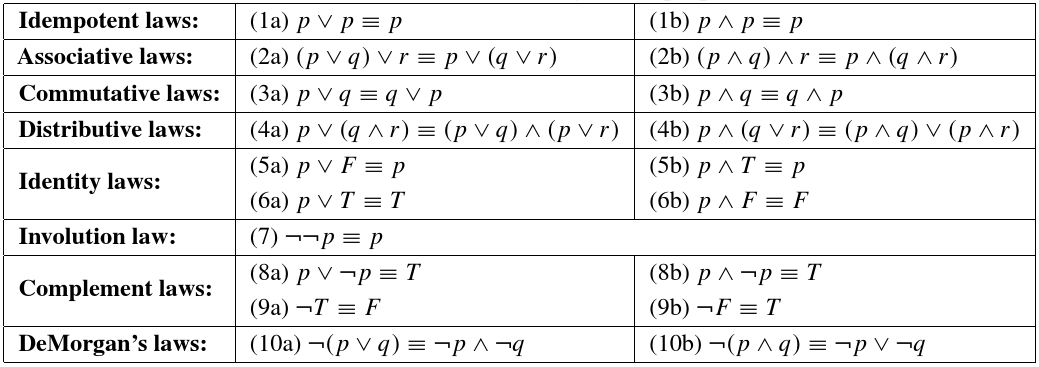
\includegraphics[width=\linewidth]{md/tabla_4-1}
 \caption{Leyes para el álgebra de proposiciones}
\label{fig:tabla:4.1}
\end{figure}



\subsection{Sentencias condicionales y bicondicionales}


 Muchas sentencias, particularmente en matemáticas, son de la forma \texttt{``si p entonces q''}.  Tales sentencias son llamadas \emph{condicionales} y son denotadas por 
 $$
 p \imply q.
 $$ 



 El condicional $p \imply q$ es frecuentemente leído como \emph{``$p$ implica $q$''} o \emph{``$p$ sólo si $q$''.}
 \sidenote{
 \begin{tdv}[Condicional]
	\begin{center}
		\begin{tabular}{|l|l||l|} \hline
			$p$ & $q$ & $p \imply q$ \\ \hline
			$1$ & $1$ & $1$ \\ \hline
			$1$ & $0$ & $0$ \\ \hline
			$0$ & $1$ & $1$ \\ \hline
			$0$ & $0$ & $1$ \\ \hline
		\end{tabular}
	\end{center}
	
\end{tdv} 
}



 Otra sentencia común es de la forma \emph{``$p$ si y solo si $q$''.}  Tales sentencias son llamadas \emph{bicondicionales} y se denota por 
 $
 p \iff q.
 $ \sidenote{ 
 \begin{tdv}[Bicondicional]
	\begin{center}
		\begin{tabular}{|l|l||l|} \hline
			$p$ & $q$ & $p \biconditional q$ \\ \hline
			$1$ & $1$ & $1$ \\ \hline
			$1$ & $0$ & $0$ \\ \hline
			$0$ & $1$ & $0$ \\ \hline
			$0$ & $0$ & $1$ \\ \hline
		\end{tabular}
	\end{center}
	
\end{tdv} 
}







 \begin{resuelto}
  Demuestre que $$p\imply q \equiv \neg p \vee q.$$
 \end{resuelto}




 \begin{resuelto} Determine cuales de las siguientes sentencias son tautologías, construyendo las correspondientes tablas de verdad.
  \begin{enumerate}
   \item $\neg\left( p \vee \neg q \right) \imply \neg p$
   \item $p \imply \left( q\imply r \right)$
   \item $\left( p \imply q \right)\imply r$
   \item $\left( p\imply q \right) \imply \left( q\imply p \right)$
   \item $\left( p \wed \left( p \imply q \right) \right) \imply q$
   \item $\left( p \wed q \right) \imply p$
   \item $q \imply \left( \neg p \vee \neg q \right)$
   \item $\left( \left( p\imply q \right) \wed \left( q \imply r \right) \right) \imply \left( p \imply r \right)$
  \end{enumerate}

 \end{resuelto}



\subsection{Argumentos}


 Un \emph{argumento} es una afirmación de que un conjunto dado de proposiciones $$P_{1}, P_{2},...,P_{n},$$ llamadas \emph{premisas}, tiene como consecuencia otra proposición $Q,$ llamada \emph{conclusión.}\sidenote{
Por ejemplo
  \begin{center}
	\begin{tabular}{l}
		Si sube el dólar, sube la gasolina.\\
		Si sube la gasolina, entonces hay inflación.\\\hline
		$\therefore$ Si sube el dólar, entonces hay inflación.
	\end{tabular}
\end{center} 
}
 
 En otras palabras, es una sentencia de la forma
 $$
  \left( P_{1} \wed P_{2} \wed...\wed P_{n}\right) \imply Q
  $$
 
 La noción de \emph{``argumento lógico''} o \emph{``argumento válido''} se formaliza de la manera siguiente:
 
 \begin{definicion}
  \label{lip:4.4}
  Un argumento se dice que es \emph{válido} si la proposición 
  $$
  \left( P_{1} \wed P_{2} \wed...\wed P_{n}\right) \imply Q
  $$ es una tautología. 
  Tal argumento se denota por $$P_{1}, P_{2},...,P_{n} \yields Q.$$
  
   Si un argumento no es \emph{válido,} diremos que es una \emph{falacia.}
 \end{definicion}




 \begin{resuelto}
 \label{lip:exmp:4.4}
  \begin{enumerate}
   \item Demuestre que $p, p\imply q \yields q$ es un argumento válido. 
   \item Demuestre que $p\imply q, q \yields p$ es una falacia.
   
   \item Demuestre que $p\imply q, \neg q \yields \neg p$ es un argumento válido.
  \end{enumerate}

 \end{resuelto}

	% TODO: \usepackage{graphicx} required
	\begin{figure}
		\centering
		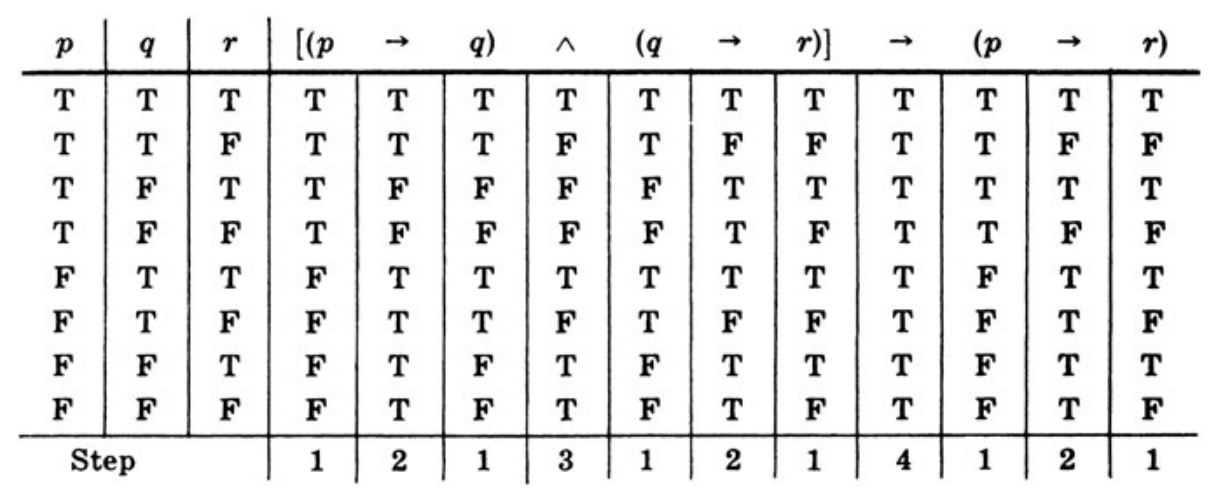
\includegraphics[width=0.7\linewidth]{md/tabla_silogismo}
		\caption{
			  Un principio fundamental del razonamiento lógico nos dice que:
				Si $p$ implica $q$ y $q$ implica $r,$ entonces $p$ implica $r.$ 
			En otras palabras, el siguiente argumento es válido
			$$
			p\imply,q, q\imply r \yields p \imply r.
			$$ }
		%\label{fig:tablasilogismo}
		\label{fig:tabla_silogismo}
	\end{figure}

\subsection{Notación de conjuntos}

Un conjunto se puede entender de forma intuitiva como una colección de objetos. Aunque la definición formal es mucho más complicada, para nuestros fines basta con esta idea sencilla.\footnote{Lee por ejemplo el artículo \href{https://www.britannica.com/science/set-theory/Axiomatic-set-theory}{Axiomatic set theory}. Para profundizar más, ve la conferencia \href{https://youtu.be/hLFit88zTYk}{¿Teoría de conjuntos? ¡Pero si es bien fácil!}, impartida en el Instituto de Matemáticas de la UNAM.}

Por convención, un conjunto se puede describir de manera \emph{extensiva} escribiendo todos y cada uno de sus elementos entre paréntesis, o bien alguna característica que los defina. Por ejemplo, el conjunto de los dígitos se puede describir como
\[
	\set{\texttt{dígitos}}=\set{0,1,2,3,4,5,6,7,8,9}=\set{0,1,...,9}.
\]

	El conjunto de los números naturales está dado por
	\[ \N = \set{0,1,2,3...} ,\]	
	mientras que los números naturales están dados por 
	\[ \Z = \set{0,\pm 1, \pm 2, \pm 3...} .\]	
	Al conjunto de enteros positivos los denotaremos por $ \Z^{+}. $
	
		Si un elemento $ x $ pertenece a un conjunto $ A $, escribiremos $ x\in A $. En caso contrario, $ x\not \in A $.

\subsection{Funciones proposicionales y Cuantificadores}


 Una \emph{función proposicional} (o \emph{sentencia abierta} o \emph{condición}) definida en un conjunto $A$ es una expresión $p(x)$ que tiene la propiedad de que $p(a)$ es cierta o falsa para cada $a \in A.$



 El conjunto $A$ se conoce como dominio de $p(x),$ y el subconjunto de todos los elementos para los cuales $p(x)$ es cierto se conoce como el \emph{conjunto de verdad} $T_{p}$ de $p(x):$
 
 $$T_{p}=\set{x \mid x\in A, p(x)=\texttt{1}},$$ 
 o simplemente 
 $$
 T_{p}=\set{x \mid p(x)}.
 $$
Esta es la manera \emph{intensiva} de describir un conjunto.



 \begin{resuelto}
  \label{lip:exmp:4.7}
  Encuentre el conjunto de verdad para cada función en $\N$:
  \begin{enumerate}
   \item $p(x): x+2>7$ 
   \item $p(x): x+5<3$ 
   \item $p(x): x+5>1$ 
  \end{enumerate}

 \end{resuelto}



\subsection{Cuantificador universal}


 Sea $p(x)$ una función proposicional definido en un conjunto $A.$ La expresión
 \[
 \label{lip:4.1}
   \forall x \in A: p(x)
 \] 
 se lee como  \texttt{``para todo $x\in A,$ $p(x)$ es verdadero.''}  Al símbolo $\forall$ (\texttt{``para todo''}) se llama cuantificador universal.

 Si $p(x)$ es una sentencia abierta (su valor de verdad depende de cada $x\in A$), la afirmación 
 $$\forall x\in A: p(x)$$ es verdadera si y solo si $p(x)$ se cumple para todo $x\in A.$  Si existe algún $x\in A$ tal que $p(x)$ es falso, entonces $$\forall x\in A: p(x)$$ es falso.



 \begin{resuelto}
  \label{lip:exmp:4.8}
  Verifique el valor de verdad de las siguientes afirmaciones:
  \begin{enumerate}
   \item $\forall n \in \N: n+4>3.$ 
   \item $\forall n \in \N: n+2>8.$
  \end{enumerate}

 \end{resuelto}



\subsection{Cuantificador existencial}


 Sea $p(x)$ una función proposicional definido en un conjunto $A.$ La expresión
 \[
 \label{lip:4.3}
   \exists x \in A: p(x)
 \] 
 se lee como  \texttt{``existe $x\in A,$ tal que $p(x)$ es verdadero.''}  
 
 El símbolo $\exists$ (\texttt{``existe...''}) se llama cuantificador existencial.




 Mientras que $p(x)$ es una sentencia abierta (su valor de verdad depende de cada $x\in A$), la afirmación 
 $$\exists x\in A: p(x)$$ es verdadera si y solo si $p(x)$ se cumple para algún elemento $x\in A.$  



 Por otro lado,  $$\exists x\in A: p(x)$$ es falso si y solo si para todo $ x\in A $, se tiene que $ p(x) $ es falso.



 Verifique el valor de verdad de las siguientes afirmaciones:
 \begin{enumerate}
  \item $\exists n  \in \N: n+4<7;$ 
  \item $\exists n \in \N: n+6<4.$
 \end{enumerate}



\subsection{Negación de Sentencias Cuantificadas}



 Considere la afirmación:
 \begin{center}
  \emph{Todos los estudiantes de ingeniería saben programar.}
 \end{center}
?`Cómo podemos negar esta afirmación?


\begin{center}
 \emph{Al menos un estudiante de ingeniería no sabe programar.}
\end{center} 


 De manera similar, la negación de la afirmación
 \begin{center}
  \emph{Existe algún estudiante de ingeniería que sepa programar}
 \end{center}
 es equivalente a afirmar que 
 \begin{center}
  \emph{Cada uno de los estudiantes de ingeniería no saben programar.}
 \end{center}

Estos son ejemplos de la siguiente proposición

 \begin{teorema}[DeMorgan]
  \begin{align}
  \label{lip:thm:4.4}
   \neg\left( \forall x\in M: p(x) \right)& \equiv \exists x\in M: \neg p(x)\\
   \label{lip:thm:4.5}
   \neg\left( \exists x\in M: p(x) \right)& \equiv \forall x\in M: \neg p(x).
  \end{align}

 \end{teorema}




 \begin{resuelto}
  \label{lip:exmp:4.10.a}
  La negación de la siguiente afirmación
  \begin{center}
   \emph{Para todo entero positivo $n,$ tenemos que $n+2>8$}
  \end{center}
es 
\begin{center}
 \emph{Existe un entero positivo $n$ tal que $n+2 \leq 8.$}
\end{center}

 \end{resuelto}




 \begin{resuelto}
  \label{lip:exmp:4.10.b}
  La negación de la siguiente afirmación
  \begin{center}
   \emph{Existe una persona viva con 150 a\~nos o más.}
  \end{center}
 es 
 \begin{center}
  \emph{Toda persona viva tiene menos de 150 a\~nos.}
 \end{center}

 \end{resuelto}

 \begin{observacion}
  Para negar una afirmación del tipo $$\forall x \in A: p(x)$$ sólo necesitamos encontrar un elemento $x_{0}\in A$ tal que $p(x)$ sea \emph{falso.}
  
  
  A un elemento $x_{0}$ así se le conoce como \emph{contraejemeplo.}
 \end{observacion}

 \begin{resuelto}
 \label{lip:4.11}
  \begin{enumerate}
   \item 
  Un contraejemplo para $\forall x \in \R: \abs{x}\neq 0$ es $x=0.$  
   \item 
  Un contraejemplo para $\forall x \in \R: x^{2}\geq x$ es $x=\frac{1}{2}.$  
   \item 
  Sin embargo, $\forall x \in \N: : x^{2}\leq x$ es siempre cierto.
  \end{enumerate}

 \end{resuelto}





%\subsection{Bibliografía}
% Las notas de esta sección están basadas en el capítulo 4 \texttt{``Logic and Propositional Calculus''} del libro
% \begin{center}
%  \texttt{Lipschutz, S. and Lipson, M.;\textbf{ Schaum's Outline of Discrete Mathematics;} McGraw-Hill, 3th Edition.}
% \end{center}
